\chapter{Applications for Regional and Global EnKF}\label{application}
\setlength{\parskip}{12pt}

In this chaper, the elements from the previous chapters will be applied to demonstrate how to run a regional and global case using the GSI observer and EnKF. These examples are intended to give users a clear idea of how to set up the GSI observer and EnKF for a particular application and properly check the run status and analysis results in order to determine if the run was successful. Note that the regional example focuses on WRF ARW, however WRF NMM and NMMB runs are similar, but require different background ensemble and namelist options. Similarly, the global example features a single global configuration (T254), however users may wish to use a different configuration, again requiring different background ensemble and namelist options.

It is assumed that the reader has successfully compiled GSI and EnKF on a local machine. 
For \textbf{regional case studies}, users should have the following data available:
\begin{enumerate}
\item Ensemble for background
\begin{itemize}
\item Ensemble files from WRF-ARW, WRF-NMM, NMM-B forecast files may be
used. For this case, WRF-ARW ensemble members will be used, which are generated from the GFS ensemble, following the naming convention: \verb|wrfarw.mem00nn|. Where \verb|nn| corresponds to each ensemble member ("ensmean" appended for ensemble mean).
\end{itemize}
\item Conventional, GPSRO and radiance data
\begin{itemize}
\item Real time GDAS and NAM PrepBUFR data can be obtained from the server:
\url{ftp://ftpprd.ncep.noaa.gov/pub/data/nccf/com/gfs/prod/}   \\
\url{ftp://ftpprd.ncep.noaa.gov/pub/data/nccf/com/nam/prod/}  \\
\end{itemize}
\item Fixed files
\begin{itemize}
\item Fixed files are located in the \verb|comGSIv3.5_EnKFv1.1/fix| directory
\end{itemize}
\end{enumerate}

For \textbf{global case studies}, users should have the following data available: 
\begin{enumerate}
\item Ensemble for background
\begin{itemize}
\item Ensemble files from GFS forecast files may be used. GFS ensemble members corresponding to various spectral resolutions may be used, following the naming convention: \verb|sfg_yyyymmddhh_fhrff_mem0nn|. The "yyyymmddhh" corresponds to the initialization date, "ff" corresponds to the forecast hour, and "nn" corresponds to each ensemble member (\verb|ensmean| appended for ensemble mean).
\end{itemize}
\item Conventional data
\begin{itemize}
\item Real time GDAS PrepBUFR (and BUFR) data can be obtained from the server:  \\
\url{ftp://ftpprd.ncep.noaa.gov/pub/data/nccf/com/gfs/prod/}
\end{itemize}
\item Fixed files
\begin{itemize}
\item Fixed files are located in the \verb|comGSIv3.5_EnKFv1.1/fix/global| directory
\end{itemize}
\end{enumerate}
The following cases will give users an example of how to run the EnKF for a regional case with various data sources, as well as a simple global application case. Users are welcome to download these examples from the EnKF User\textquotesingle s webpage (online case for release v1.1) or create a new background ensemble and obtain observation data from the above server.

The background ensemble files and observations used in the regional case studies are as follows:
\begin{enumerate}
\item Background files: wrfarw.mem0001 - wrfarw.mem0020, wrfarw.ensmean
\begin{itemize}
\item The horizontal grid spacing is 45-km with 51 vertical sigma levels.
% figure 5.1
% Background used for regional case study
\begin{figure}[h!]
  \centering
  \caption{Background used for regional case study}
  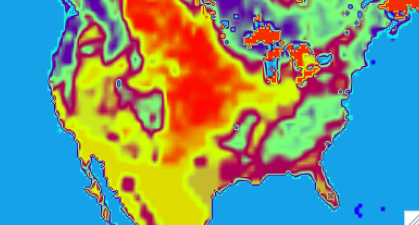
\includegraphics[width=0.7\textwidth]{images/ch5_figure1.jpg} 
 \label{ch5_fig1}
\end{figure}
\end{itemize}
\item Conventional, GPSRO and radiance data from 00 UTC 13 February 2014
\begin{itemize}
\item Conventional file:  
\begin{itemize}
\item \verb|gdas1.t00z.prepbufr.nr|
\end{itemize}
\item GPSRO file: 
\begin{itemize}
\item \verb|gdas1.t00z.gpsro.tm00.bufr_d| 
\end{itemize}
\item Radiance files: 
\begin{itemize}
\item \verb|gdas1.t00z.1bamua.tm00.bufr_d| 
\item \verb|gdas1.t00z.1bhrs4.tm00.bufr_d| 
\item \verb|gdas1.t00z.1bmhs.tm00.bufr_d| 
\end{itemize}
\end{itemize}
\item Fixed files:
\begin{itemize}
\item Fixed files are located in the GSI/EnKF community code package, under
\verb|/comGSIv3.5_EnKFv1.1/fix|
\item For observation control:
\begin{itemize}
\item \verb|convinfo|: conventional data (PrepBUFR, GPSRO) info file 
\item \verb|ozinfo|: ozone retrival info file
\item \verb|satinfo|: satellite radiance info file 
\end{itemize}
\item Adaptive radiance bias correction (although example files are provided in the \verb|/fix| directory, it is better to obtain bias correction files valid for the proper date. For this case, GFS bias correction coefficients are provided with the case data):
\begin{itemize} 
\item \verb|satbias_in|: satellite bias correction coefficient file
\item \verb|satbias_pc|: satellite bias correction coefficient file for passive channels.
\end{itemize}
\end{itemize}
\end{enumerate}



This case study was run on a linux cluster. GSI no longer (from GSI v3.2) requires byte- swapping to little endian format. BUFRLIB can automatically handle byte order issues.

For the \textbf{regional ARW case}, assume the following locations:

Path to the background ensemble files:
\begin{verbatim}
       /scratch/casedata/arw_2014021300/bk/
\end{verbatim}
the path to the observations:
\begin{verbatim}
       /scratch/casedata/arw_2014021300/obs
\end{verbatim}
and the GSI release version 3.5/EnKF version 1.1 is located at:
\begin{verbatim}
       /scratch/comGSIv3.5_EnKFv1.1
\end{verbatim}
For the global GFS case, assume locations as follows: Path to background ensemble files:
\begin{verbatim}
       /scratch/casedata/enkf_glb_t254/bk
\end{verbatim}
the path to the observations:
\begin{verbatim}
       /scratch/casedata/enkf_glb_t254/obs
\end{verbatim}
and the GSI release version 3.5/EnKF version 1.1 is located at:
\begin{verbatim}
       /scratch/comGSIv3.5_EnKFv1.1
\end{verbatim}


%----------------------------------------------
\section{Running GSI Observer for Regional Applications}
%----------------------------------------------

%----------------------------------------------
\subsection{Run Script}
%----------------------------------------------

With both GSI and EnKF compiled and the background ensemble files and observations acquired, 
the next step is to work with the gsi observer run script, \verb|run_gsi_regional.ksh|. The location of this 
script is under \verb|comGSIv3.5_EnKFv1.1/run|. This run script is the same as the one used for 
a GSI analysis run, with a few specific options selected in order to loop through all the ensemble 
members and generate the ensemble observation priors for each member and the ensemble 
mean. In addition to the GSI observer specific options, other user-specific modifications need 
to be made:

\begin{itemize}
\item \textbf{Set up batch queueing system} \\
To run GSI with multiple processors, a job queuing head must be added to the \verb| run_gsi_regional.ksh | script. The set up of the job queue is dependent on the machine and the job control system. Refer to the GSI User\textquotesingle s
 Guide, section 3.2.2, for more examples of the setup section of this script. The following example is setup to run on a Linux cluster with LSF:
\begin{footnotesize}
\begin{verbatim}
#BSUB -P ??????             # project code
#BSUB -W 00:30                 # wall-clock time (hrs:mins)
#BSUB -n 4                  # number of tasks in job         
#BSUB -R "span[ptile=16]"      # run 16 MPI tasks per node
#BSUB -J gsi                   # job name
#BSUB -o gsi.%J.out          # output file name in which %J is replaced by the job ID
#BSUB -e gsi.%J.err          # error file name in which %J is replaced by the job ID
#BSUB -q small               # queue
\end{verbatim}
\end{footnotesize}

\item \textbf{Set up number of processors and the job queue system used} 
For this example, \verb|LINUX_LSF| and 4 processors are used:

\begin{footnotesize}
\begin{verbatim}
     GSIPROC=4 
     ARCH='LINUX_LSF'
\end{verbatim}
\end{footnotesize}

\item \textbf{Set up the case data, analysis time, fix files, GSI executable, and CRTM coefficients:} 

Set up analysis time:

\begin{footnotesize}
\begin{verbatim}
     ANAL_TIME=2014021300
\end{verbatim}
\end{footnotesize}

Set up working directory, which will hold the analysis results (all ensemble members will be run in this directory). This directory must have the proper write permissions as well as enough space to hold the output.

\begin{footnotesize}
\begin{verbatim}
     WORK_ROOT=/scratch/${user}/comGSIv3.5_EnKFv1.1/run/gsidiag_2014021300
\end{verbatim}
\end{footnotesize}

Set path to the observation directory and the PrepBUFR file within the observation directory. All observations to be assimilated should reside in this directory.

\begin{footnotesize}
\begin{verbatim}
     OBS_ROOT=/scratch/${user}/casedata/arw_2014021300/obs 
     PREPBUFR=${OBS_ROOT}/gdas1.t00z.prepbufr.nr
\end{verbatim}
\end{footnotesize}

Set path to background ensemble files:

\begin{footnotesize}
\begin{verbatim}
     BK_ROOT=/scratch/${user}/casedata/arw_2014021300/bk
\end{verbatim}
\end{footnotesize}

Set file for background ensemble mean:

\begin{footnotesize}
\begin{verbatim}
     BK_FILE=${BK_ROOT}/wrfarw.ensmean
\end{verbatim}
\end{footnotesize}

Set the GSI system used for this case, including the paths of the fix files and the CRTM coefficents as well as the location of the GSI executable:

\begin{footnotesize}
\begin{verbatim}
     CRTM_ROOT=/scratch/${user}/CRTM_REL-2.2.3 
     GSI_ROOT=/scratch/${user}/comGSIv3.5_EnKFv1.1/ 
     FIX_ROOT=${GSI_ROOT}/fix 
     GSI_EXE=${GSI_ROOT}/run/gsi.exe 
     GSI_NAMELIST=${GSI_ROOT}/run/comgsi_namelist.sh
\end{verbatim}
\end{footnotesize}

\item \textbf{Set which background and background error file to use}

\begin{footnotesize}
\begin{verbatim}
     bk_core=ARW 
     bkcv_option=NAM 
     if_clean=clean
\end{verbatim}
\end{footnotesize}

This example uses the ARW NetCDF background; therefore \verb| bk_core | is set to \verb|ARW|. The regional background error covariance file is used in this case, as set by \verb| bkcv_option=NAM |. Finally, the run scripts are set to clean the run directory to delete all temporary intermediate files.\\

\item \textbf{Choose to run GSI observer, set up background ensemble information}

\begin{footnotesize}
\begin{verbatim}
     if_observer=Yes
     no_member=20 
     BK_FILE_mem=${BK_ROOT}/wrfarw.mem
\end{verbatim}
\end{footnotesize}

The option \verb|if_observer=Yes| is the switch that enables \verb|run_gsi_regional.ksh| to run the GSI observer (rather than GSI analysis). In this example, 20 ensemble members are selected with the naming convention: 
\verb|wrfarw.memnnnn|. Note that memnnnn which is associated with each ensemble member (nnnn), is not included and will be appended later in the script.\\

\item \textbf{Link observations} 

\begin{footnotesize}
\begin{verbatim}
# Link to the prepbufr data
ln -s ${PREPBUFR} ./prepbufr
# Link to the radiance data
ln -s ${OBS_ROOT}/gdas1.t00z.1bamua.tm00.bufr_d amsuabufr 
ln -s ${OBS_ROOT}/gdas1.t00z.1bhrs4.tm00.bufr_d hirs4bufr 
ln -s ${OBS_ROOT}/gdas1.t00z.1bmhs.tm00.bufr_d mhsbufr
ln -s ${OBS_ROOT}/gdas1.t00z.gpsro.tm00.bufr_d gpsrobufr
\end{verbatim}
\end{footnotesize}

\end{itemize}

Past the arch selection, environment variable checks, and creation of working directory, users will find the location where the observations are linked. For this case, we can see that the conventional PrepBUFR observations have been linked, as well as three different satellite radiance BUFR files (AMSU-A, HIRS4, and MHS) and a GPS RO BUFR file. These files will be linked to the working directory and separate observation innovation (diag) files will be generated for each observation.

In the run script, the proper anavinfo file is selected based on the core and background error covariance used for the case:

\begin{footnotesize}
\begin{verbatim}
  echo ' Use NAM background error covariance'
  BERROR=${FIX_ROOT}/${BYTE_ORDER}/nam_nmmstat_na.gcv
  OBERROR=${FIX_ROOT}/nam_errtable.r3dv
  if [ ${bk_core} = NMM ] ; then
     ANAVINFO=${FIX_ROOT}/anavinfo_ndas_netcdf
  fi
  if [ ${bk_core} = ARW ] ; then
     ANAVINFO=${FIX_ROOT}/anavinfo_arw_netcdf
  fi
  if [ ${bk_core} = NMMB ] ; then
     ANAVINFO=${FIX_ROOT}/anavinfo_nems_nmmb
  fi
\end{verbatim}
\end{footnotesize}

The anavinfo file used for this case is \verb| anavinfo_arw_netcdf |, because the background is NetCDF ARW and the regional background error covariance has been selected. It is
important to check this file, located in the \verb|./fix| directory. The number of vertical levels in  \verb| anavinfo_arw_netcdf | must match those for the background. In this example, the case has 50 vertical levels with the default value in \verb|anavinfo_arw_netcdf| is 40. Change these values (\verb|level column|) accordingly:

\begin{footnotesize}
\begin{verbatim}
met_guess::
!var     level    crtm_use    desc              orig_name
  ps        1      -1         surface_pressure     ps
  z         1      -1         geopotential_height  phis
  u        50       2         zonal_wind           u
  v        50       2         meridional_wind      v
  div      50      -1         zonal_wind           div
  vor      50      -1         meridional_wind      vor
  tv       50       2         virtual_temperature  tv
  q        50       2         specific_humidity    sphu
  oz       50       2         ozone                ozone
  cw       50      10         cloud_condensate     cw
... ...
control_vector::
!var     level  itracer as/tsfc_sdv  an_amp0   source  funcof
 sf       50      0       1.00        -1.0     state    u,v
 vp       50      0       1.00        -1.0     state    u,v
 ps        1      0       0.50        -1.0     state    prse
 t        50      0       0.70        -1.0     state    tv
 q        50      1       0.70        -1.0     state    q
 oz       50      1       0.50        -1.0     state    oz
 sst       1      0       1.00        -1.0     state    sst
 cw       50      1       1.00        -1.0     state    cw
 stl       1      0       1.00        -1.0     motley   sst
 sti       1      0       1.00        -1.0     motley   sst
::
\end{verbatim}
\end{footnotesize}

%----------------------------------------------
\subsection{Run GSI Observer and Check Run Status}
%----------------------------------------------

Once the run script is set up properly for the case and the machine, GSI can be run through the run script. The following command will submit the job:
\begin{small}
\begin{verbatim}
$ bsub < run_gsi_regional.ksh
\end{verbatim}
\end{small}

While the job is running, move to the working directory and check the details. Given the following working directory setup:

\begin{small}
\begin{verbatim}
WORK_ROOT=/scratch/${user}/comGSIv3.5_EnKFv1.1/run/gsidiag_2014021300
\end{verbatim}
\end{small}

Go to directory \verb|WORK_ROOT=/scratch/${user}/comGSIv3.5_EnKFv1.1/| and check the run directory. A directory named \verb|gsidiag_2014021300| should have been created. This directory is the run directory for this GSI observer case study. The directory will be populated with many files:

\begin{footnotesize}
\begin{verbatim}
amsua_n18.TauCoeff.bin 
ssmi_f15.SpcCoeff.bin 
amsua_n18.SpcCoeff.bin 
ssmi_f15.TauCoeff.bin 
imgr_g11.SpcCoeff.bin
imgr_g11.TauCoeff.bin
\end{verbatim}
\end{footnotesize}

These files are CRTM coefficients that have been linked to this run directory through the GSI run script. Similar to running the GSI analysis, many other files are linked or copied to this run directory, such as:

\begin{table}[htbp]
\centering
\begin{tabular}{ll}

\textit{gsiparm.anl}: & GSI namelist \\

\textit{prepbufr}: & PrepBUFR file for conventional observation \\

\textit{convinfo}: & data usage control for conventional data   \\

\textit{satbias\_in}: & satellite bias correction coefficient file   \\

\textit{satinfo}: & data usage and channel control for satellite radiance data \\ 
  
\textit{berror\_stats}: & background error file  \\
 
\textit{errtable}: & observation error file \\
            
\end{tabular}
\end{table}

Additionally, for the GSI observer many files are generated as a result of the \verb|lread_obs_save| and \verb|lread_obs_skip| options in the namelist for writing/reading collective observation selection information:

\begin{table}[htbp]
\centering
\begin{tabular}{ll}

\textit{obs\_input.nnnn}: & During ensemble mean (save=True, skip=False), save all observation \\
                                       & preprocessing to this file. Each file (nnnn) is for a different variable type\\
                                      

\textit{pennnn.obs\_setup}: &  When looping through ensemble members (save=False, skip=True), \\
                                            & all observation preprocessing is skipped, \textit{obs\_input.nnnn} files \\
                                            & are read and \textit{pennnn.obs\_setup} is written for each processor \\
                                            & (nnnn) for all observations.

\end{tabular}
\end{table}

As the GSI observer is running for the ensemble mean as well as looping through each member, files are are generated for each ensemble member, as well as the ensemble mean.
\begin{table}[htbp]
\centering
\begin{tabular}{ll}
\textit{pennnn.conv\_01}: & Files generated after O-B, generated for conventional  \\
                                         & observations as well as one file per sensor (e.g. AMSU-A n18).   \\
                                         & These files are trimmed for resulting diag files and cleaned.\\
\textit{list\_run\_directory}: & Directory listing after ensemble mean is run, before directory \\
                                          & is cleaned for running the ensemble members.\\
\textit{list\_run\_directory\_memnnn}:  & As as above, for each ensemble member (nnn).\\
\textit{stdout}:  &  Standard output file for ensemble mean.\\                                                  
\textit{stdout\_memnnn}: & Standard output file for each ensemble member (nnn).\\
\end{tabular}
\end{table}

The presence of the standard output files in the directory suggest the GSI observer run scripts have successfully set up a run environment for the GSI observer, properly looping through the ensemble members, and the GSI executable is running on each ensemble member. 

Once GSI has finished running, diag files should be generated for each observation type for each member as well as the ensemble mean:
\begin{footnotesize}
\begin{verbatim}
diag_conv_ges.ensmean    diag_conv_ges.mem001
diag_conv_ges.mem002     diag_conv_ges.mem003
diag_conv_ges.mem004     diag_conv_ges.mem005
... ...                  diag_conv_ges.mem020

diag_amsua_metop-a_ges.ensmean diag_amsua_metop-a_ges.mem001
diag_amsua_metop-a_ges.mem002  diag_amsua_metop-a_ges.mem003
diag_amsua_metop-a_ges.mem004  diag_amsua_metop-a_ges.mem005
 ... ...                       diag_amsua_metop-a_ges.mem020

diag_amsua_n18_ges.ensmean      diag_amsua_n18_ges.mem001
diag_amsua_n18_ges.mem002       diag_amsua_n18_ges.mem003
diag_amsua_n18_ges.mem004       diag_amsua_n18_ges.mem005
......
diag_hirs4_n19_ges.ensmean          diag_amsua_n15_ges.mem001
diag_hirs4_n19_ges.mem002           diag_amsua_n15_ges.mem003
diag_hirs4_n19_ges.mem004           diag_amsua_n15_ges.mem005
... ...                             diag_amsua_n15_ges.mem020

\end{verbatim}
\end{footnotesize}



%----------------------------------------------
\subsection{Check for Successful GSI Completion}
%----------------------------------------------

The presence of the diag files and standard out files for the ensemble mean and each member indicates that the GSI observer has run without crashing, but does not necessary indicate a successful analysis. It is important to check the stdout files in the run directory to make sure the GSI observer completed each step without any obvious problems. The following are several important areas of the standard out file to check:
\begin{enumerate}
\item Read in the anavinfo and namelist
\begin{footnotesize}
\begin{verbatim}
 gsi_metguess_mod*init_:  2D-MET STATE VARIABLES:
 ps
 z
 gsi_metguess_mod*init_:  3D-MET STATE VARIABLES:
 u
 v
 div
 vor
 tv
 q
 oz
 cw
.....

 &SETUP
 GENCODE =   78.0000000000000     ,
 FACTQMIN        =  0.000000000000000E+000,
 FACTQMAX        =  0.000000000000000E+000,
.....
\end{verbatim}
\end{footnotesize}

\item Read in the background field

The following lines in stdout immediately following the namelist section, indicate that GSI is reading the background fields. Checking that the range of the max and min values will indicate if particular background fields are normal.

\begin{footnotesize}
\begin{verbatim}
  dh1  =            3
  iy,m,d,h,m,s=        2014           2          13           0           0
           0
  dh1  =            3
 rmse_var = SMOIS
 ndim1 =            3
 ordering = XYZ
 staggering =  N/A
 start_index =            1           1           1           0
 end_index =          129          70           4           0
 WrfType =          104
 ierr  =            0
... ...
  rmse_var = T ndim1=           3
  WrfType =          104  WRF_REAL=         104 ierr  =            0
  ordering = XYZ staggering =  N/A
  start_index =            1           1           1           0  end_index =
         129          70          50           0
  k,max,min,mid T=           1   313.3391       237.9947       273.2565
  k,max,min,mid T=           2   313.4587       238.4884       273.5590
  k,max,min,mid T=           3   313.6850       239.3906       274.1599
  k,max,min,mid T=           4   314.0594       241.0577       275.0899
  k,max,min,mid T=           5   314.6113       243.6186       276.3394
  k,max,min,mid T=           6   315.3213       247.0504       277.7711
... ...
\end{verbatim}
\end{footnotesize}

\item Read in observational data

The \verb|stdout| (ensemble mean) and \verb|stdout_memnnn| (ensemble members) contains distinct differences for the reading in the observational data controlled by the \verb|lread_obs_save| and \verb|lread_obs_skip| options in the namelist \\

a. Ensemble mean
\begin{scriptsize}
\begin{verbatim}
 read_obs_check: bufr file date is   2014021300 prepbufr q
 read_obs_check: bufr file date is   2014021300 prepbufr ps
 read_obs_check: bufr file uv                   not available satwndbufr
 read_obs_check: bufr file rw                   not available radarbufr
 read_obs_check: bufr file pcp_tmi   trmm       not available tmirrbufr
 read_obs_check: bufr file hirs3     n17        not available hirs3bufr
... ...
  number of extra processors            1
 READ_OBS:  read   33 mhs        mhs_n18              using ntasks=   2   0   1795      0
 READ_OBS:  read   34 mhs        mhs_n19              using ntasks=   2   2    584      0
 READ_OBS:  read   35 mhs        mhs_metop-a          using ntasks=   2   0    174      0
 READ_OBS:  read   36 mhs        mhs_metop-b          using ntasks=   2   2      2      0
... ...
 READ_BUFRTOVS         : file=mhsbufr         type=mhs        sis=mhs_n19              nread=         0
 ithin= 2 rmesh=  60.000000 isfcalc= 0 ndata=         0 ntask=  2
... ...
 READ_PREPBUFR         : file=prepbufr        type=uv         sis=uv                   nread=     52122
 ithin= 0 rmesh= 120.000000 isfcalc= 0 ndata=     50772 ntask=  1
... ...
 READ_OBS:  write collective obs selection info to obs_input.common
\end{verbatim}
\end{scriptsize}

For the ensemble mean, the same procedure for observation processing as the GSI analysis is followed (\verb|read_obs_check|, \verb|READ_OBS|, \verb|READ_BUFRTOVS|, \verb|READ_GPS|, \verb|READ_PREPBUFR| ...). Finally, it is indicated that the collective observations selection information is written out for use with the ensemble members.\\

b. Ensemble members

For the \verb|stdout_memnnn|, the observation processing steps are skipped and observation information is read in from the ensemble mean:

\begin{footnotesize}
\begin{verbatim}
OBSERVER_SET: read collective obs selection info from obs_input.common
\end{verbatim}
\end{footnotesize}


Finally, for both the ensemble mean and members, the following lines will appear:
\begin{footnotesize}
\begin{verbatim}
OBS_PARA: ps                        2038      2538      5499      6600
OBS_PARA: t                         3271      4431      7459      8753
OBS_PARA: q                         2823      3917      6110      7187
OBS_PARA: pw                         261       217       226       180
OBS_PARA: uv                        3333      5207      9038      8902
OBS_PARA: gps_ref                    597      1001       210      1085
OBS_PARA: hirs4     metop-a            0         0         0       174
OBS_PARA: amsua     n15              542       540         0         0
OBS_PARA: amsua     n18              606       672         0         0
OBS_PARA: amsua     metop-a            0         0         0       151
OBS_PARA: mhs       n18              730       828         0         0
OBS_PARA: mhs       metop-a            0         0         0       201
\end{verbatim}
\end{footnotesize}

This table is important to check if the observations have been read in, which types of observations have been read in, and the distribution of observations in each subdomain.\\

\item Indication that the GSI observer has successfully run:
\begin{footnotesize}
\begin{verbatim}
 observer_final: successfully finalized
 glbsoi: complete
[000]gsisub(): : complete.


     ENDING DATE-TIME    JUL 14,2016  23:29:19.825  196  THU   2457584
     PROGRAM GSI_ANL HAS ENDED.
* . * . * . * . * . * . * . * . * . * . * . * . * . * . * . * . * . * . * . * .
\end{verbatim}
\end{footnotesize}

\end{enumerate}

After looking over each section of the standard output files, it can be concluded that the GSI observer ran without issues. Note that because the outer loop was set to 0 (\verb|miter=0|) for the GSI observer, no minimization occurred and therefore no analysis results were produced.
   
%----------------------------------------------
\section{Running EnKF for Regional Applications}
%----------------------------------------------

%----------------------------------------------
\subsection{Run Script}
%----------------------------------------------

Once the GSI observer has been run successfully, the next step is to setup the EnKF run script, \verb|run_enkf_wrf.ksh|. This script is located under \verb|comGSIv3.5_EnKFv1.1/run|. This run script uses the diag files generated by the GSI observer script as observation input, and generates the EnKF analysis. Similar to the GSI observer script, several user-specific modifications need to be made:
\begin{itemize}
\item Set up batch queueing system
\begin{footnotesize}
\begin{verbatim}
#BSUB -P ????             # project code
#BSUB -W 00:30                 # wall-clock time (hrs:mins)
#BSUB -n 32                  # number of tasks in job         
#BSUB -R "span[ptile=16]"      # run 16 MPI tasks per node
#BSUB -J gsi                   # job name
#BSUB -o gsi.%J.out          # output file name in which %J is replaced by the job ID
#BSUB -e gsi.%J.err          # error file name in which %J is replaced by the job ID
#BSUB -q small               # queue
\end{verbatim}
\end{footnotesize}

\item Set up number of processors and the job queue system used:
\begin{footnotesize}
\begin{verbatim}
  GSIPROC=32
  ARCH='LINUX_LSF'
\end{verbatim}
\end{footnotesize}
One difference from the GSI observer script is that the number of processors used should be greater than at least the number of ensemble members for running the EnKF. In this case we have 20 ensemble members and have requested 32 cores.\\

\item Set up the analysis time, fixed files, EnKF executable
\begin{footnotesize}
\begin{verbatim}
  ANAL_TIME=2014021300
  WORK_ROOT=/scratch/${user}/comGSIv3.5_EnKFv1.1/run/enkf_2014021300
  diag_ROOT=/scratch/${user}/comGSIv3.5_EnKFv1.1/run/gsidiag_2014021300
  BK_ROOT=/scratch/${user}/casedata/arw_2014021300/bk
  BK_FILE=${BK_ROOT}/wrfarw.ensmean
  GSI_ROOT=/scratch/${user}/comGSIv3.5_EnKFv1.1
  FIX_ROOT=${GSI_ROOT}/fix
  ENKF_EXE=${GSI_ROOT}/src/main/enkf/wrf_enkf
  CRTM_ROOT=/scratch/${user}/CRTM_2.2.3/
  ENKF_NAMELIST=${GSI_ROOT}/run/enkf_wrf_namelist.sh
\end{verbatim}
\end{footnotesize}

\item Set background file and location of the diag files (from GSI observer)

\begin{footnotesize}
\begin{verbatim}
    diag_ROOT=/scratch/${user}/comGSIv3.5_EnKFv1.1/run/gsidiag_2014021300
    BK_FILE=${BK_ROOT}/wrfarw.ensmean
\end{verbatim}
\end{footnotesize}

Two modifications to note for the EnKF are the \verb|diag_ROOT| and \verb|BK_FILE|. The \verb|diag_ROOT| points to the working directory where the GSI observer was run. This directory contains diag* files which will be linked to the EnKF working directory. \verb|BK_FILE| points to the background ensemble mean.\\

\item Select ensemble parameters

\begin{footnotesize}
\begin{verbatim}
  NMEM_ENKF=20
  BK_FILE_mem=${BK_ROOT}/wrfarw
  NLONS=129
  NLATS=70
  NLEVS=50
  IF_ARW=.true.
  IF_NMM=.false.
\end{verbatim}
\end{footnotesize}

The next section sets information about the ensemble, including the number of members, background ensemble members, domain specifications, dynamical core, and list of observations to be used in the EnKF. Note that the ensemble members (\verb|BK_FILE_mem|) do not include the 3-digit member number. This will be appended to the name specified for this field later in the script.\\

\item Select observations
\begin{verbatim}
       list="conv amsua_n18 amsua_metop-a"
\end{verbatim}
\end{itemize}
The previous line is contained with the ensemble parameter section. For the observations to be assimilated, be aware that only observations/platforms that have been run through the GSI observer (and therefore a diag* file exists) are valid.

%----------------------------------------------
\subsection{Run EnKF and Check Run Status}
%----------------------------------------------

Once the run script is set up properly for the case and the machine, EnKF can be run through the run script. The following command will submit the job:
\begin{small}
\begin{verbatim}
     $ bsub < run_enkf_wrf.ksh
\end{verbatim}
\end{small}

While the job is running, move to the working directory and check the details. Given the following working directory setup:
\begin{small}
\begin{verbatim}
  WORK_ROOT=/scratch/${user}/comGSIv3.5_EnKFv1.1/run/enkf_2014021300
\end{verbatim}
\end{small}

Go to directory \verb|/scratch/${user}/comGSIv3.5_EnKFv1.1/run| and check the run directory. A directory named \verb|enkf_2014021300| should have been created. This directory is the run directory for this EnKF case study. The directory will be populated with many links:
\begin{footnotesize}
\begin{verbatim}
diag_conv_ges.ensmean  diag_conv_ges.mem007  diag_conv_ges.mem014
diag_conv_ges.mem001   diag_conv_ges.mem008  diag_conv_ges.mem015
diag_conv_ges.mem002   diag_conv_ges.mem009  diag_conv_ges.mem016
diag_conv_ges.mem003   diag_conv_ges.mem010  diag_conv_ges.mem017
diag_conv_ges.mem004   diag_conv_ges.mem011  diag_conv_ges.mem018
diag_conv_ges.mem005   diag_conv_ges.mem012  diag_conv_ges.mem019
diag_conv_ges.mem006   diag_conv_ges.mem013  diag_conv_ges.mem020

diag_amsua_n18_ges.ensmean  diag_amsua_n18_ges.mem007  diag_amsua_n18_ges.mem014
diag_amsua_n18_ges.mem001   diag_amsua_n18_ges.mem008  diag_amsua_n18_ges.mem015
diag_amsua_n18_ges.mem002   diag_amsua_n18_ges.mem009  diag_amsua_n18_ges.mem016
diag_amsua_n18_ges.mem003   diag_amsua_n18_ges.mem010  diag_amsua_n18_ges.mem017
diag_amsua_n18_ges.mem004   diag_amsua_n18_ges.mem011  diag_amsua_n18_ges.mem018
diag_amsua_n18_ges.mem005   diag_amsua_n18_ges.mem012  diag_amsua_n18_ges.mem019
diag_amsua_n18_ges.mem006   diag_amsua_n18_ges.mem013  diag_amsua_n18_ges.mem020

diag_hirs4_metop-a_ges.ensmean  diag_hirs4_metop-a_ges.mem007  diag_hirs4_metop-a_ges.mem014
diag_hirs4_metop-a_ges.mem001   diag_hirs4_metop-a_ges.mem008  diag_hirs4_metop-a_ges.mem015
diag_hirs4_metop-a_ges.mem002   diag_hirs4_metop-a_ges.mem009  diag_hirs4_metop-a_ges.mem016
diag_hirs4_metop-a_ges.mem003   diag_hirs4_metop-a_ges.mem010  diag_hirs4_metop-a_ges.mem017
diag_hirs4_metop-a_ges.mem004   diag_hirs4_metop-a_ges.mem011  diag_hirs4_metop-a_ges.mem018
diag_hirs4_metop-a_ges.mem005   diag_hirs4_metop-a_ges.mem012  diag_hirs4_metop-a_ges.mem019
diag_hirs4_metop-a_ges.mem006   diag_hirs4_metop-a_ges.mem013  diag_hirs4_metop-a_ges.mem020
\end{verbatim}
\end{footnotesize}

The diag files are linked from the GSI observer working directory. These links are specified in the run script. Note that ozone diag files (gome, omi, sbuv) will appear in the directory without links (zero length files) if ozone diags are not present from the GSI observer.

The first guess files are also linked into the directory from the run script, pointing to the path of the ensemble mean and ensemble members designated in the setup section.
\begin{footnotesize}
\begin{verbatim}
firstguess.ensmean  firstguess.mem007  firstguess.mem014
firstguess.mem001   firstguess.mem008  firstguess.mem015
firstguess.mem002   firstguess.mem009  firstguess.mem016
firstguess.mem003   firstguess.mem010  firstguess.mem017
firstguess.mem004   firstguess.mem011  firstguess.mem018
firstguess.mem005   firstguess.mem012  firstguess.mem019
firstguess.mem006   firstguess.mem013  firstguess.mem020
\end{verbatim}
\end{footnotesize}


Similar to running the GSI observer, many other static files are linked or copied to this run directory, such as:
\begin{table}[htbp]
\centering
\begin{tabular}{ll}
\textit{enkf.nml}: & EnKF namelist \\
\textit{convinfo}: & data usage control for conventional data \\
\textit{satbias\_in}:& satellite bias correction coefficient file\\
\textit{satbias\_pc}: &satellite bias correction file for passive channels \\
\textit{satinfo}: & data usage and channel control for satellite radiance data\\
\textit{ozinfo}: & data usage control from ozone data\\
\textit{covinflate.dat}: & Three-dimensional multiplicative inflation factor fields\\
\textit{stdout}: & EnKF standard output file\\
\end{tabular}
\end{table}

 The presence of the standard output file in the directory suggest the EnKF run script has successfully set up a run environment for the EnKF, properly linking the first guess and diag files from the GSI observer, and the EnKF executable is running. Once EnKF has finished running, analysis files should be generated for each member as well as the ensemble mean:
 \begin{footnotesize}
 \begin{verbatim}
analysis.ensmean  analysis.mem006  analysis.mem012  analysis.mem018
analysis.mem001   analysis.mem007  analysis.mem013  analysis.mem019
analysis.mem002   analysis.mem008  analysis.mem014  analysis.mem020
analysis.mem003   analysis.mem009  analysis.mem015  
analysis.mem004   analysis.mem010  analysis.mem016
analysis.mem005   analysis.mem011  analysis.mem017
\end{verbatim}
\end{footnotesize}
   
%----------------------------------------------
\subsection{Check for Successful EnKF Completion}
%----------------------------------------------

The presence of the analysis files for the ensemble mean and each member as well as the standard out file indicates that the EnKF has run without crashing, but does not necessary indicate a successful analysis. It is important to check the stdout file in the run directory to make sure the EnKF completed each step without any obvious problems. The following are several important areas of the standard out file to check:

\begin{enumerate}
\item Check namelist has been properly read in and configuration is correct:

\begin{footnotesize}
\begin{verbatim}
 namelist parameters:
 --------------------
 &NAM_ENKF
 DATEIN  =  2014021300,
 DATAPATH        = ./                                                                                       
 IASSIM_ORDER    =           0,
 COVINFLATEMAX   =   100.0000    ,
 COVINFLATEMIN   =   1.000000    ,
 DETERMINISTIC   = T,
... ...
\end{verbatim}
\end{footnotesize}

\item Check number of ensemble members, as well as the actual analysis variables and the background type. The maximum and minimum values for surface pressure are printed for a sanity check:

\begin{footnotesize}
\begin{verbatim}
          20  members
 number of background forecast times to be updated =            1
 first-guess forecast hours for analysis = 06
           5 3d vars to update
 total of         251  2d grids will be updated (including ps)
 using multiplicative inflation based on Pa/Pb
 Vars in Rad-Jacobian (dims)
 --------------------------
 sst                            0
 enkf_main:  number of threads            1
 Updating U, V, T, QVAPOR, PH, and MU for WRF-ARW...
 Surface pressure (spressmn) min/max range:   678.673339843750
   1032.22473144531
\end{verbatim}
\end{footnotesize}

\item Statistics of the ensemble prior\\
Following many lines describing the bias correction coefficients, the inventory of the observation number, observation types from the input diag* files, and the time spent reading in each observation type, statistics of the ensemble priors fit to all observations are provided for each region (NH, SH, TR):

\begin{footnotesize}
\begin{verbatim}
 innovation statistics for prior:
 conventional obs
 region, obtype, nobs, bias, innov stdev, sqrt(S+R), sqrt(S), sqrt(R):
NH    all ps  14083 -0.591E-02  0.860E+00  0.814E+00  0.601E+00  0.550E+00
TR    all ps     50 -0.629E-01  0.422E+00  0.661E+00  0.367E+00  0.550E+00
NH     all t   7766 -0.228E+00  0.163E+01  0.128E+01  0.480E+00  0.119E+01
TR     all t    138 -0.130E+00  0.118E+01  0.119E+01  0.234E+00  0.117E+01
NH    all uv  21680  0.136E-01  0.295E+01  0.276E+01  0.140E+01  0.237E+01
TR    all uv    302 -0.379E+00  0.251E+01  0.268E+01  0.124E+01  0.238E+01
NH     all q   2553 -0.323E-01  0.146E+00  0.157E+00  0.868E-01  0.131E+00
TR     all q     68 -0.721E-01  0.202E+00  0.164E+00  0.582E-01  0.154E+00
 satellite brightness temp
 instrument, channel #, nobs, bias, innov stdev, sqrt(S+R), sqrt(S), sqrt(R):
           amsua_n18   1   241 -0.199E+00  0.194E+01  0.306E+01  0.176E+01  0.250E+01
           amsua_n18   2   248 -0.194E+00  0.145E+01  0.234E+01  0.806E+00  0.220E+01
           amsua_n18   3   248 -0.620E+00  0.119E+01  0.206E+01  0.497E+00  0.200E+01
           amsua_n18   4   248 -0.189E+00  0.398E+00  0.568E+00  0.140E+00  0.550E+00
           amsua_n18   5   248  0.188E-01  0.337E+00  0.315E+00  0.966E-01  0.300E+00
           amsua_n18   6  1203 -0.396E-01  0.198E+00  0.238E+00  0.610E-01  0.230E+00
           amsua_n18   7  1225 -0.215E+00  0.324E+00  0.235E+00  0.480E-01  0.230E+00
           amsua_n18   8  1155 -0.235E+00  0.369E+00  0.259E+00  0.675E-01  0.250E+00
           amsua_n18  10  1211  0.408E+00  0.491E+00  0.353E+00  0.429E-01  0.350E+00
           amsua_n18  11    12  0.720E+00  0.723E+00  0.404E+00  0.567E-01  0.400E+00
           amsua_n18  15   245 -0.311E+00  0.198E+01  0.380E+01  0.148E+01  0.350E+01
       hirs4_metop-a   3     1  0.115E+01  0.115E+01  0.534E+00  0.631E-01  0.530E+00
       hirs4_metop-a   4    42  0.260E+00  0.521E+00  0.403E+00  0.488E-01  0.400E+00
       hirs4_metop-a   5     7 -0.534E+00  0.558E+00  0.367E+00  0.696E-01  0.360E+00
       hirs4_metop-a   6     7 -0.748E+00  0.782E+00  0.473E+00  0.109E+00  0.460E+00
       hirs4_metop-a   7     9 -0.557E+00  0.815E+00  0.580E+00  0.108E+00  0.570E+00
       hirs4_metop-a   8     9  0.374E+00  0.675E+00  0.100E+01  0.208E-01  0.100E+01
       hirs4_metop-a  10     9  0.199E+00  0.581E+00  0.612E+00  0.120E+00  0.600E+00
       hirs4_metop-a  11     9 -0.380E-01  0.718E+00  0.143E+01  0.770E+00  0.120E+01
       hirs4_metop-a  12    34 -0.988E+00  0.179E+01  0.213E+01  0.141E+01  0.160E+01
       hirs4_metop-a  13     9  0.694E-01  0.330E+00  0.382E+00  0.116E+00  0.364E+00
       hirs4_metop-a  14     9 -0.369E-01  0.257E+00  0.294E+00  0.137E+00  0.260E+00
       hirs4_metop-a  15     9  0.352E-01  0.289E+00  0.281E+00  0.107E+00  0.260E+00
\end{verbatim}
\end{footnotesize}

This table should be checked in order to determine if the inflation is appropriate. The goal is to make the total ensemble spreads of priors ($\sqrt{S+R}$ match the innovations (innov std) as much as possible. We can see in certain regions, particularly in the NH the differences are noteable. These differences are associated with higher observation error ($\sqrt{R}$). Users should consider tuning of inflation and localization, which is typically determined using cases with multiple assimilation cycles. Refer to section 4.2 of this User\textquotesingle s Guide for more information on tuning.\\

\item Domain and observation partition:

\begin{footnotesize}
\begin{verbatim}
 npts =         9030
 min/max number of points per proc =          243         317
 time to do model space decomp =   1.529277069494128E-003
 nobstot =        53078
 min/max number of obs per proc =         1658        1659
 time to do ob space decomp =   3.935033455491066E-004
 sending out observation prior ensemble perts from root ...
 nobstot*nanals               1061560
 npts*ndim               2266530
 ... took   1.730861375108361E-002  secs
 time in load_balance =  7.929413160309196E-002 on proc           0
\end{verbatim}
\end{footnotesize}


The analysis variables and the observations are distributed to different processors. We can see in this case that the min/max number of points per processor are 243 and 317, respectively. Similarly, we can see that the min/max number of observations per processor are 1658 and 1659, respectively, indicating that the observations are well dispersed among the processors.

\begin{footnotesize}
\begin{verbatim}
 READGRIDDATA_ARW: U           1  -20.55222       20.72632
 READGRIDDATA_ARW: U           2  -20.87878       21.20316
 READGRIDDATA_ARW: U           3  -21.61046       22.36177
 READGRIDDATA_ARW: U           4  -22.62561       24.08465
 READGRIDDATA_ARW: U           5  -24.07165       26.47827
 READGRIDDATA_ARW: U           6  -25.89237       32.81841
 READGRIDDATA_ARW: U           7  -27.10455       35.81213
... ...
\end{verbatim}
\end{footnotesize}

Additionally, check the minimum and maximum values of the fields at each vertical level as a quick sanity check.

\end{enumerate}

%----------------------------------------------
\subsection{Diagnose EnKF Analysis Results}
%----------------------------------------------

At the bottom of the standard output file, there are several output statistics and tables that are helpful for users to diagnose the quality of the EnKF analysis.\\
\begin{enumerate}
\item Spread inflation of the analysis ensemble

\begin{footnotesize}
\begin{verbatim}
 global ps prior std. dev min/max =    21.52301       172.3270
 NH mean ps prior standard deviation =    57.82042
 NH mean ps posterior standard deviation (before inflation)=    29.20955
 NH mean ps posterior standard deviation (after inflation) =    54.58403
 NH mean ps inflation =    2.421974
 TR mean ps prior standard deviation =    31.09247
 TR mean ps posterior standard deviation (before inflation)=    28.31872
 TR mean ps posterior standard deviation (after inflation) =    30.79383
 TR mean ps inflation =    1.106122
 time in inflate_ens =  1.366839744150639E-002 on proc           0
\end{verbatim}
\end{footnotesize}

This section is important for checking whether the values of the inflation are reasonable by looking at a summary of the maximum and minimum values. Also, viewing the regional averaged statistics before and after inflation. For this case we can see both the NH and TR show larger standard deviation after the inflation, which is more consistent with the prior standard deviation. \\

\item Spread inflation of the analysis ensemble
\begin{footnotesize}
\begin{verbatim}
 innovation statistics for posterior:
 conventional obs
 region, obtype, nobs, bias, innov stdev, sqrt(S+R), sqrt(S), sqrt(R):
NH    all ps  14083  0.503E-03  0.757E+00  0.569E+00  0.146E+00  0.550E+00
TR    all ps     50 -0.562E-01  0.398E+00  0.585E+00  0.198E+00  0.550E+00
NH     all t   7766 -0.780E-01  0.145E+01  0.122E+01  0.263E+00  0.119E+01
TR     all t    138 -0.107E+00  0.115E+01  0.118E+01  0.199E+00  0.117E+01
NH    all uv  21680  0.406E-01  0.267E+01  0.246E+01  0.655E+00  0.237E+01
TR    all uv    302 -0.259E+00  0.236E+01  0.246E+01  0.636E+00  0.238E+01
NH     all q   2553 -0.174E-01  0.114E+00  0.138E+00  0.444E-01  0.131E+00
TR     all q     68 -0.279E-01  0.168E+00  0.159E+00  0.413E-01  0.154E+00
 satellite brightness temp
 instrument, channel #, nobs, bias, innov stdev, sqrt(S+R), sqrt(S), sqrt(R):
           amsua_n18   1   241  0.614E+02  0.915E+02  0.263E+01  0.823E+00  0.250E+01
           amsua_n18   2   248 -0.132E+03  0.171E+03  0.223E+01  0.376E+00  0.220E+01
           amsua_n18   3   248 -0.303E+02  0.398E+02  0.201E+01  0.244E+00  0.200E+01
           amsua_n18   4   248 -0.231E+00  0.580E+01  0.555E+00  0.776E-01  0.550E+00
           amsua_n18   5   248 -0.788E+00  0.199E+01  0.305E+00  0.575E-01  0.300E+00
           amsua_n18   6  1203 -0.138E+01  0.158E+01  0.234E+00  0.423E-01  0.230E+00
           amsua_n18   7  1225 -0.273E+01  0.287E+01  0.232E+00  0.322E-01  0.230E+00
           amsua_n18   8  1155 -0.131E+01  0.186E+01  0.254E+00  0.437E-01  0.250E+00
           amsua_n18  10  1211 -0.179E+01  0.196E+01  0.352E+00  0.374E-01  0.350E+00
           amsua_n18  11    12 -0.130E+01  0.133E+01  0.404E+00  0.537E-01  0.400E+00
           amsua_n18  15   245 -0.163E+03  0.198E+03  0.357E+01  0.693E+00  0.350E+01
       hirs4_metop-a   3     1  0.118E+01  0.118E+01  0.533E+00  0.558E-01  0.530E+00
       hirs4_metop-a   4    42  0.286E+00  0.542E+00  0.403E+00  0.455E-01  0.400E+00
       hirs4_metop-a   5     7 -0.451E+00  0.487E+00  0.364E+00  0.562E-01  0.360E+00
       hirs4_metop-a   6     7 -0.724E+00  0.755E+00  0.468E+00  0.852E-01  0.460E+00
       hirs4_metop-a   7     9 -0.572E+00  0.817E+00  0.577E+00  0.871E-01  0.570E+00
       hirs4_metop-a   8     9  0.122E+01  0.136E+01  0.100E+01  0.205E-01  0.100E+01
       hirs4_metop-a  10     9  0.855E+00  0.100E+01  0.609E+00  0.104E+00  0.600E+00
       hirs4_metop-a  11     9 -0.236E-01  0.543E+00  0.130E+01  0.507E+00  0.120E+01
       hirs4_metop-a  12    34 -0.738E+00  0.153E+01  0.178E+01  0.790E+00  0.160E+01
       hirs4_metop-a  13     9  0.121E+01  0.128E+01  0.375E+00  0.905E-01  0.364E+00
       hirs4_metop-a  14     9  0.776E-01  0.256E+00  0.281E+00  0.106E+00  0.260E+00
       hirs4_metop-a  15     9  0.281E+00  0.384E+00  0.273E+00  0.838E-01  0.260E+00
\end{verbatim}
\end{footnotesize}

After the EnKF analysis, it is important to check the innovation statistics, much like the prior fit to all observation.
\end{enumerate}

%----------------------------------------------
% section
\section{Running GSI Observer for Global Applications}
%----------------------------------------------

%----------------------------------------------
\subsection{Run Script}
%----------------------------------------------

With both GSI and EnKF compiled (note that a separate global executable must be generated for EnKF) and the background ensemble files and observations acquired, the next step is to work with the gsi observer run script, \verb|run_gsi_global.ksh|. The location of this script is under \verb|comGSIv3.5_EnKFv1.1/run|. This run script is the same as the one used for a GSI global analysis run, with a few specific options selected in order to loop through all the ensemble members and generate the ensemble observation priors for each member and the ensemble mean. For the global examples, users must choose a case that corresponds to the spectral resolution of the background ensemble. For this example, we will be using T254. In addition to the GSI observer specific options, other user-specific modifications need to be made:

\begin{itemize}
\item Set up batch queueing system \\
To run GSI with multiple processors, a job queuing head must be added to the \verb|run_gsi_global.ksh| script. The set up of the job queue is dependent on the machine and the job control system. Refer to the GSI User\textquotesingle s Guide, section 3.2.2, for more examples of the setup section of this script. The following example is setup to run on a Linux cluster with LSF:

\begin{footnotesize}
\begin{verbatim}
# LSF batch script to run an MPI application
#BSUB -P ???????             # project code
#BSUB -W 00:30                 # wall-clock time (hrs:mins)
#BSUB -n 24                   # number of tasks in job         
#BSUB -R "span[ptile=16]"      # run 16 MPI tasks per node
#BSUB -J gsi                   # job name
#BSUB -o gsi.%J.out          # output file name in which %J is replaced by the job ID
#BSUB -e gsi.%J.err          # error file name in which %J is replaced by the job ID
#BSUB -q small               # queue
\end{verbatim}
\end{footnotesize}

\item Set up number of processors and the job queue system used. For this example, \verb|LINUX_LSF| and 24 processors are used:

\begin{footnotesize}
\begin{verbatim}
  GSIPROC=24
  ARCH='LINUX_LSF'
\end{verbatim}
\end{footnotesize}

\item Set up the case data, analysis time, fix files, GSI executable, and CRTM coefficients:  \\

Set up analysis time and select global case:

\begin{footnotesize}
\begin{verbatim}
  ANAL_TIME=2014040512
  GFSCASE=enkf_glb_t254
\end{verbatim}
\end{footnotesize}

Set up working directory, which will hold the analysis results (all ensemble members will be run in this directory). This directory must have the proper write permissions as well as enough space to hold the output.

\begin{footnotesize}
\begin{verbatim}
WORK_ROOT=/scratch/${user}/comGSIv3.5-EnKFv1.1/run/gsidiag_${GFS_CASE}
\end{verbatim}
\end{footnotesize}

Set path to background ensemble files:

\begin{footnotesize}
\begin{verbatim}
BK_ROOT=/scratch/${user}/casedata/enkf_glb_t254/bk
\end{verbatim}
\end{footnotesize}

Set path to the observation directory and the PrepBUFR file within the observation directory. All observations to be assimilated should reside in this directory.

\begin{footnotesize}
\begin{verbatim}
OBS_ROOT=/scratch/${user}/casedata/enkf_glb_t254/obs 
PREPBUFR=${OBS_ROOT}/gdas1.t12z.prepbufr.nr
\end{verbatim}
\end{footnotesize}

Set the GSI system used for this case, including the paths of the fix files and the CRTM coefficients as well as the location of the GSI executable:

\begin{footnotesize}
\begin{verbatim}
CRTM_ROOT=/scratch/${user}/CRTM_REL-2.2.3 
GSI_ROOT=/scratch/${user}/comGSIv3.5_EnKFv1.1/ 
FIX_ROOT=${GSI_ROOT}/fix 
GSI_EXE=${GSI_ROOT}/run/gsi.exe 
GSI_NAMELIST=${GSI_ROOT}/run/comgsi_namelist_gfs.sh
\end{verbatim}
\end{footnotesize}

Note that the GSI namelist generation script used for the global case (\verb|comgsi_namelist_gfs.sh|) is different from the one used for the regional example.\\

\item Choose to run GSI observer, set up background ensemble information

\begin{footnotesize}
\begin{verbatim}
  if_observer=Yes  # Yes ,or, No -- case sensitive!!!
  no_member=10
  BK_FILE_mem=${BK_ROOT}/sfg_2014040506
\end{verbatim}
\end{footnotesize}

The option \verb|if_observer=Yes| is the switch that enables \verb|run_gsi_global.ksh| to run the GSI observer (rather than GSI analysis). In this example, 10 ensemble members are selected with the naming convention: \verb|sfg_${GUESS_DATE}_memnnnn| . Note that \verb|_memnnnn| which is assocated with each ensemble member (\verb|nnnn|), is not included and will be appended later in the script.\\

\item  Set the JCAP resolution for the case:
\begin{footnotesize}
\begin{verbatim}
if [[ "$GFSCASE" = "T62" ]]; then
  JCAP=62
  JCAP_B=62
elif [[ "$GFSCASE" = "T126" ]]; then
  JCAP=126
  JCAP_B=126
elif [[ "$GFSCASE" = "enkf_glb_t254" ]]; then
  JCAP=254
  JCAP_B=254
elif [[ "$GFSCASE" = "T254" ]]; then
  JCAP=254
  JCAP_B=574
elif [[ "$GFSCASE" = "T574" ]]; then
  JCAP=574
  JCAP_B=1534
else
   echo "INVALID case = $GFSCASE"
   exit
fi
  LEVS=64
\end{verbatim}
\end{footnotesize}
Note that this selection is filled based on selection of the GFSCASE. This example used the \verb|enkf_glb_t254| case. All cases use 64 levels. \\

Further in the run script \verb|run_gsi_global.ksh|, the resolution parameters are set based on the requested case (resolution). For this case, we are using JCAP=254:
\begin{footnotesize}
\begin{verbatim}
elif [[ "$JCAP" = "254" ]]; then
   LONA=512
   LATA=256
   DELTIM=1200
   resol=2
\end{verbatim}
\end{footnotesize}


\item Link satellite bias correction coefficients, background ensemble files, and observations:
\begin{footnotesize}
\begin{verbatim}
if [[ "$GFSCASE" = "enkf_glb_t254" ]]; then
  cp $OBS_ROOT/gdas1.t12z.abias      ./satbias_in
  cp $OBS_ROOT/gdas1.t12z.satang     ./satbias_angle

  cp $BK_ROOT/sfcanl_2014040506_fhr03_ensmean  ./sfcf03
  cp $BK_ROOT/sfcanl_2014040506_fhr06_ensmean  ./sfcf06
  cp $BK_ROOT/sfcanl_2014040506_fhr06_ensmean  ./sfcf09

  cp $BK_ROOT/sfg_2014040506_fhr03_mem001    ./sigf03
  cp $BK_ROOT/sfg_2014040506_fhr06_mem001    ./sigf06
  cp $BK_ROOT/sfg_2014040506_fhr09_mem001    ./sigf09
... ...
# Link to the prepbufr data
ln -s ${PREPBUFR} ./prepbufr

# Link to the other observation data

if [[ "$GFSCASE" = "enkf_glb_t254" ]]; then
  obsfile_amua=gdas1.t12z.1bamua.tm00.bufr_d
  obsfile_amub=gdas1.t12z.1bamub.tm00.bufr_d
else
\end{verbatim}
\end{footnotesize}
Past the arch selection, environment variable checks, and creation of working directory, users will find the location where the observations are linked. For this case, we can see that the conventional PrepBUFR observations have been linked, as well as AMSU-A and AMSU-B satellite radiance BUFR files. These files will be linked to the working directory and separate observation innovation (\verb|diag|) files will be generated for each observation.
\end{itemize}

%
%----------------------------------------------
\subsection{Run GSI Observer and Check Run Status}
%----------------------------------------------

Once the run script is set up properly for the case and the machine, GSI can be run through the run script. The following command will submit the job:

\begin{footnotesize}
\begin{verbatim}
$ bsub < run_gsi_global.ksh
\end{verbatim}
\end{footnotesize}

While the job is running, move to the working directory and check the details. Given the following working directory setup:
\begin{footnotesize}
\begin{verbatim}
WORK_ROOT=/scratch/${user}/comGSIv3.5_EnKFv1.1/run/gsidiag_${GFSCASE}
\end{verbatim}
\end{footnotesize}
Go to directory \verb|/scratch/${user}/comGSIv3.5_EnKFv1.1/| and check the run directory. A directory named \verb|gsidiag_enkf_glb_t254| should have been created. This directory is the run directory for this GSI observer case study. The directory will be populated with many files such as:

\begin{footnotesize}
\begin{verbatim}
AerosolCoeff.bin                 hirs4_n19.TauCoeff.bin         sndrD1_g14.TauCoeff.bin
ahi_himawari8.SpcCoeff.bin       iasi616_metop-a.SpcCoeff.bin   sndrD1_g15.SpcCoeff.bin
ahi_himawari8.TauCoeff.bin       iasi616_metop-a.TauCoeff.bin   sndrD1_g15.TauCoeff.bin
airs281SUBSET_aqua.SpcCoeff.bin  iasi616_metop-b.SpcCoeff.bin   sndrD2_g11.SpcCoeff.bin
... ...
\end{verbatim}
\end{footnotesize}

These files are CRTM coefficients that have been linked to this run directory through the GSI run script. Similar to running the GSI analysis, many other files are linked or copied to this run directory, such as:

\begin{table}[htbp]
\centering
\begin{tabular}{ll}
\verb|gsiparm.anl| :   & GSI namelist   \\
\verb|prepbufr| :   &  PrepBUFR file for conventional observation \\
\verb|convinfo| :   &  data usage control for conventional data \\
\verb|satbias_in| :   &  satellite bias correction coefficient file  \\
\verb|satinfo| :   &   data usage and channel control for satellite radiance data \\
\verb|berror_stats| :   &  background error file \\
\verb|errtable| :    &    observation error file \\
\end{tabular}
\end{table}
% table
Additionally, for the GSI observer many files are generated as a result of the \verb|lread_obs_save| and \verb|lread_obs_skip| options in the namelist for writing/reading collective observation selection information:
%table
\begin{table}[htbp]
\centering
\begin{tabular}{ll}
\verb|obs_input.nnnn|:  & During ensemble mean (save=True, skip=False), save all observation  \\
                                      & preprocessing to this file. Each file (nnnn) is for a different variable type \\
\verb|pennnn.obs_setup|:  &  When looping through ensemble members (save=False, skip=True), \\
                                          & all observation preprocessing is skipped, \verb|obs_input.nnnn| files \\
                                          & are read and \verb|pennnn.obs_setup| is written for each processor \\
                                          & (nnnn) for all observations.\\ 
\end{tabular}
\end{table}
% table

As the GSI observer is running for the ensemble mean as well as looping through each member, files are for each ensemble member, as well as the ensemble mean: \\

%table
\begin{table}[htbp]
\centering
\begin{tabular}{ll}
\verb|pennnn.conv_01| : & Files generated after O-B, generated for conventional \\
                                        & observations as well as one file per sensor (e.g. AMSU-A n18). \\
                                         & These files are trimmed for resulting \verb|diag| files and cleaned. \\
\verb|list_run_directory| : &   Directory listing after ensemble mean is run, before directory \\
                                            & is cleaned for running the ensemble members.\\
\verb|list_run_directory_memnnn|:  &    As as above, for each ensemble member (nnn).\\
\verb|stdout | : &  Standard output file for ensemble mean. \\
\verb|stdout_memnnn| : &     Standard output file for each ensemble member (nnn).\\
\end{tabular}
\end{table}
% table
The presence of the standard output files in the directory suggest the GSI observer run scripts have successfully set up a run environment for the GSI observer, properly looping through the ensemble members, and the GSI executable is running on each ensemble member. Once GSI has finished running, \verb|diag| files should be generated for each observation type for each member as well as the ensemble mean:

\begin{footnotesize}
\begin{verbatim}
diag_conv_ges.ensmean  diag_conv_ges.mem004  diag_conv_ges.mem008
diag_conv_ges.mem001   diag_conv_ges.mem005  diag_conv_ges.mem009
diag_conv_ges.mem002   diag_conv_ges.mem006  diag_conv_ges.mem010
diag_conv_ges.mem003   diag_conv_ges.mem007
diag_amsua_metop-a_ges.ensmean  diag_amsua_metop-a_ges.mem006
diag_amsua_metop-a_ges.mem001   diag_amsua_metop-a_ges.mem007
diag_amsua_metop-a_ges.mem002   diag_amsua_metop-a_ges.mem008
diag_amsua_metop-a_ges.mem003   diag_amsua_metop-a_ges.mem009
diag_amsua_metop-a_ges.mem004   diag_amsua_metop-a_ges.mem010
diag_amsua_metop-a_ges.mem005
diag_amsua_n18_ges.ensmean  diag_amsua_n18_ges.mem004  diag_amsua_n18_ges.mem008
diag_amsua_n18_ges.mem001   diag_amsua_n18_ges.mem005  diag_amsua_n18_ges.mem009
diag_amsua_n18_ges.mem002   diag_amsua_n18_ges.mem006  diag_amsua_n18_ges.mem010
diag_amsua_n18_ges.mem003   diag_amsua_n18_ges.mem007
diag_amsua_n19_ges.ensmean  diag_amsua_n19_ges.mem004  diag_amsua_n19_ges.mem008
diag_amsua_n19_ges.mem001   diag_amsua_n19_ges.mem005  diag_amsua_n19_ges.mem009
diag_amsua_n19_ges.mem002   diag_amsua_n19_ges.mem006  diag_amsua_n19_ges.mem010
diag_amsua_n19_ges.mem003   diag_amsua_n19_ges.mem007
\end{verbatim}
\end{footnotesize}

%----------------------------------------------
\subsection{Check for Successful GSI Completion}
%----------------------------------------------

The presence of the \verb|diag| files and standard out files for the ensemble mean and each member indicates that the GSI observer has run without crashing, but does not necessary indicate a successful analysis. It is important to check the stdout files in the run directory to make sure the GSI observer completed each step without any obvious problems. The following are several important areas of the standard out file to check:
\begin{enumerate}
\item Read in the \verb|anavinfo| and namelist 

\begin{footnotesize}
\begin{verbatim}
 READ_FILES:  analysis date,minutes         2014           4           5
          12           0    19070640
 gsi_metguess_mod*init_:  2D-MET STATE VARIABLES:
 ps
 z
 gsi_metguess_mod*init_:  3D-MET STATE VARIABLES:
 u
 v
... ...

 &SETUP
 GENCODE =   78.0000000000000     ,
 FACTQMIN        =  0.000000000000000E+000,
 FACTQMAX        =  0.000000000000000E+000,
\end{verbatim}
\end{footnotesize}

\item Read in the background field  \\
The following lines in the stdout immediately following the namelist section, indicate that GSI is reading the background fields. Checking that the range of the max and min values will indicate if particular background fields are normal.

\begin{scriptsize}
\begin{verbatim}
GESINFO:  jcap_b= 254, levs= 64, latb=  256, lonb=  512, ntrac=  3, ncldt=  1, idvc=  2, nvcoord=  2, 
idvm=  0, idsl=  0, idpsfc=  0, idthrm=  0
   k,ak,bk,ck,tref=  1   0.00000000000       1.00000000000       0.00000000000       300.000000000 
   k,ak,bk,ck,tref=  2   0.00000000000      0.994671165943       0.00000000000       300.000000000 
   k,ak,bk,ck,tref=  3  0.574999988079E-03  0.988626599312       0.00000000000       300.000000000 
   k,ak,bk,ck,tref=  4  0.574100017548E-02  0.981742262840       0.00000000000       300.000000000 
   ... ...
\end{verbatim}
\end{scriptsize}

\item Read in observational data \\

The \verb|stdout| (ensemble mean) and \verb|stdout_memnnn| (ensemble members) contains distinct differences for the reading in the observational data controlled by the \verb|lread_obs_save| and \verb|lread_obs_skip| options in the namelist.\\
\begin{description}
\item[ c.] Ensemble mean
\begin{scriptsize}
\begin{verbatim}
 read_obs_check: bufr file date is   2014040512 prepbufr t
 read_obs_check: bufr file date is   2014040512 prepbufr uv
 read_obs_check: bufr file date is   2014040512 prepbufr q
 read_obs_check: bufr file date is   2014040512 prepbufr ps
... ...
  number of extra processors           13
 READ_OBS:  read    1 ps         ps                   using ntasks=   1   0      0      0
 READ_OBS:  read    2 t          t                    using ntasks=   1   1      0      0
 READ_OBS:  read    3 q          q                    using ntasks=   1   2      0      0
 READ_OBS:  read    4 pw         pw                   using ntasks=   1   3   2738      0
... ...
 READ_PREPBUFR         : file=prepbufr        type=pw         sis=pw                   nread=       345 
 ithin= 0 rmesh=1450.000000 isfcalc= 0 ndata=       345 ntask=  1
 READ_BUFRTOVS         : file=amsuabufr       type=amsua      sis=amsua_n18            nread=    202575 
 ithin= 2 rmesh=1500.000000 isfcalc= 0 ndata=       675 ntask=  1
 ... ...
 READ_OBS:  write collective obs selection info to obs_input.common
\end{verbatim}
\end{scriptsize}

For the ensemble mean, the same procedure for observation processing as the GSI analysis is followed (\verb|read_obs_check|, \verb|READ_OBS|, \verb|READ_BUFRTOVS|, \verb|READ_GPS|, \verb|READ_PREPBUFR|, \ldots). Finally, it is indicated that the collective observations selection information is written out for use with the ensemble members.\\


\item[d.] Ensemble members \\
For the \verb|stdout_memnnn|, the observation processing sets are skipped and observation information is read in from the ensemble mean:
\begin{footnotesize}
\begin{verbatim}
 OBSERVER_SET:  read collective obs selection info from obs_input.common
\end{verbatim}
\end{footnotesize}

Finally, for both the ensemble mean and members, the following lines will appear:

\begin{tiny}
\begin{verbatim}
OBS_PARA: ps                          24       400      1649      2577        58       245      1496       506
                  82       402       616       251        36        67       328       864        44       224
                5210      1397        69       414       506       629
OBS_PARA: t                           48       403      3406      4875       174       488      4128      1825
                  84       724      2702      1146         4       215       882      2218       151       913
               11864      3167       160      1622      1308      2381
OBS_PARA: q                           16       370      3025      4749       154       383      3211      1737
                  51       594      2126      1102         0       161       697      1951       140       850
               10310      2974       155      1525      1104      1506
OBS_PARA: pw                           0         0         0         0         0         0         0         0
                   0         0         3         0         0         0        42        25         0         0
                 251        32         0         0         0         4
OBS_PARA: uv                          52       410      4459      5664       239      1023      4994      1835
                  86      1553      3792      1316         3       184       877      2242       180      1576
               11854      3595       264      3186      2231      2895
OBS_PARA: amsua     n15                0         0         0         0         7         9         0         0
                   1         0         0         0         5         0         0         0         3        10
                   7         0         0         0         0         0
OBS_PARA: amsua     n18                3         1         0         0         5         2         0         0
                   1         0         0         0         5         6         2         0         2         5
                   6         8         0         0         0         0
OBS_PARA: amsua     n19                0         0         3         7         0         0         0         0
                   3         1         0         0         2         9        10         6         0         0
                   0         3         0         0         0         3
OBS_PARA: amsua     metop-a            0         0         0         4         0         0         0         2
                   0         4         9         5         0         0         0         0         0         0
                   0         0         0         6         9         6
OBS_PARA: amsua     metop-b            0         0         0         0         1         0         0         0
                   6         9         0         0         3         0         0         0         4         0
                   0         0         4        11         7         0
\end{verbatim}
\end{tiny}

This table is important to check if the observations have been read in, which types of observations have been read in, and the distribution of observations in each subdomain.\\
\end{description}

\item Indication that the GSI observer has successfully run:\\

\begin{footnotesize}
\begin{verbatim}
 glbsoi: complete
[000]gsisub(): : complete.


     ENDING DATE-TIME    JUL 15,2016  15:48:52.880  197  FRI   2457585
     PROGRAM GSI_ANL HAS ENDED.
* . * . * . * . * . * . * . * . * . * . * . * . * . * . * . * . * . * . * . * .
\end{verbatim}
\end{footnotesize}
\end{enumerate}

After looking over each section of the standard output files, it can be concluded that the GSI global observer ran without issues. Note that because the outer loop was set to 0 (\verb|miter=0|) for the GSI observer, no minimization occurred and therefore no analysis results were produced.

%----------------------------------------------
\section{Running EnKF for Global Applications}
%----------------------------------------------

%----------------------------------------------
\subsection{Run Script}
%----------------------------------------------

Once the GSI global observer has been run successfully, the next step is to setup the EnKF run script, \verb|run_enkf_global.ksh|. This script is located under \verb|comGSIv3.5_EnKFv1.1/run|. This run script uses the \verb|diag| files generated by the GSI global observer script as observation input, and generates the global EnKF analysis. Similar to the GSI observer script, several user-specific modifications need to be made:
\begin{itemize}
\item Set up batch queueing system
\begin{footnotesize}
\begin{verbatim}
#BSUB -P ??????             # project code
#BSUB -W 00:30                 # wall-clock time (hrs:mins)
#BSUB -n 80                   # number of tasks in job         
#BSUB -R "span[ptile=16]"      # run 16 MPI tasks per node
#BSUB -J gsi                   # job name
#BSUB -o gsi.%J.out          # output file name in which %J is replaced by the job ID
#BSUB -e gsi.%J.err          # error file name in which %J is replaced by the job ID
#BSUB -q small               # queue
\end{verbatim}
\end{footnotesize}

One difference from the GSI observer script is that the number of processors used should be greater than at least the number of ensemble members for running the EnKF. In this case we have 10 ensemble members and have requested 80 cores due to the large global domain.\\

\item Set up the analysis time, global case, fixed files, EnKF executable
\begin{footnotesize}
\begin{verbatim}
  ANAL_TIME=2014040512
  GUESS_TIME=2014040506
  GFSCASE=enkf_glb_t254
  WORK_ROOT=/scratch/${user}/comGSIv3.5_EnKFv1.1/run/enkf_${GFSCASE} 
  BK_ROOT=/scratch/${user}/casedata/enkf_glb_t254/bk
  GSI_ROOT=/scratch/${user}/comGSIv3.5_EnKFv1.1
  FIX_ROOT=${GSI_ROOT}/fix
  ENKF_EXE=${GSI_ROOT}/src/main/enkf/global_enkf
  CRTM_ROOT=/scratch/${user}/CRTM_2.2.3
  ENKF_NAMELIST=${GSI_ROOT}/run/enkf_gfs_namelist.sh
\end{verbatim}
\end{footnotesize}

\item Set location of the diag files (from GSI observer)

\begin{footnotesize}
\begin{verbatim}
  DIAG_ROOT=/scratch/${user}/comGSIv3.5_EnKFv1.1/run/gsidiag_${GFSCASE}
\end{verbatim}
\end{footnotesize}

One modifications to note for the EnKF is the \verb|DIAG_ROOT|. The \verb|DIAG_ROOT| points to the working directory where the GSI observer runs. This directory contains \verb|diag*| files which will be linked to the EnKF working directory.\\

\item Select ensemble and case parameters

\begin{footnotesize}
\begin{verbatim}
NMEM_ENKF=10
LEVS=64
NVARS=5
... ...
elif [[ "$GFSCASE" = "enkf_glb_t254" ]]; then
  JCAP=254
  JCAP_B=254
... ...
  elif [[ "$JCAP" = "254" ]]; then
   LONA=512
   LATA=256
   DELTIM=1200
   resol=2
\end{verbatim}
\end{footnotesize}
This section sets information about the number of background ensemble members, domain specifications. This information mirrors that of the \verb|run_gsi_global.ksh| script.\\

\item Read in namelist

\begin{footnotesize}
\begin{verbatim}
#Build EnKF namelist on-the-fly
. $ENKF_NAMELIST
cat << EOF > enkf.nml

 $enkf_namelist

EOF
\end{verbatim}
\end{footnotesize}

Similar to the regional enkf (\verb|run_enkf_wrf.ksh|), the global EnKF builds the namelist from an outside script for namelist generation (\verb|enkf_gfs_namelist.sh|).\\

\item Select observations
\begin{footnotesize}
\begin{verbatim}
list="conv amsua_metop-a amsua_n18 amsua_n15"
\end{verbatim}
\end{footnotesize}
The previous line is contained within the ensemble looping section. For the observations to be assimilated, be aware that only observations/platforms that have been run through the GSI observer (and therefore a \verb|diag*| file exists) are valid. For this example case, we will only run EnKF for conventional observations.
\end{itemize}

% subsection 
%----------------------------------------------
\subsection{Run EnKF and Check Run Status}
%----------------------------------------------

Once the run script is set up properly for the case and the machine, EnKF can be run through the run script. The following command will submit the job:

\begin{footnotesize}
\begin{verbatim}
$ bsub < run_enkf_global.ksh
\end{verbatim}
\end{footnotesize}
While the job is running, move to the working directory and check the details. Given the following working directory setup:
\begin{footnotesize}
\begin{verbatim}
WORK_ROOT=/scratch/${user}/comGSIv3.5_EnKFv1.1/run/enkf_${GFSCASE}
\end{verbatim}
\end{footnotesize}

Go to directory \verb|/scratch/${user}/comGSIv3.5_EnKFv1.1/| and check the run directory. A directory named \verb|enkf_enkf_glb_t264| should have been created. This directory is the run directory for this EnKF case study. The directory will be populated with many links:
\begin{footnotesize}
\begin{verbatim}
diag_conv_ges.ensmean  diag_conv_ges.mem004  diag_conv_ges.mem008
diag_conv_ges.mem001   diag_conv_ges.mem005  diag_conv_ges.mem009
diag_conv_ges.mem002   diag_conv_ges.mem006  diag_conv_ges.mem010
diag_conv_ges.mem003   diag_conv_ges.mem007
diag_amsua_metop-a_ges.ensmean  diag_amsua_metop-a_ges.mem006
diag_amsua_metop-a_ges.mem001   diag_amsua_metop-a_ges.mem007
diag_amsua_metop-a_ges.mem002   diag_amsua_metop-a_ges.mem008
diag_amsua_metop-a_ges.mem003   diag_amsua_metop-a_ges.mem009
diag_amsua_metop-a_ges.mem004   diag_amsua_metop-a_ges.mem010
diag_amsua_metop-a_ges.mem005
diag_amsua_n18_ges.ensmean  diag_amsua_n18_ges.mem004  diag_amsua_n18_ges.mem008
diag_amsua_n18_ges.mem001   diag_amsua_n18_ges.mem005  diag_amsua_n18_ges.mem009
diag_amsua_n18_ges.mem002   diag_amsua_n18_ges.mem006  diag_amsua_n18_ges.mem010
diag_amsua_n18_ges.mem003   diag_amsua_n18_ges.mem007
diag_amsua_n19_ges.ensmean  diag_amsua_n19_ges.mem004  diag_amsua_n19_ges.mem008
diag_amsua_n19_ges.mem001   diag_amsua_n19_ges.mem005  diag_amsua_n19_ges.mem009
diag_amsua_n19_ges.mem002   diag_amsua_n19_ges.mem006  diag_amsua_n19_ges.mem010
diag_amsua_n19_ges.mem003   diag_amsua_n19_ges.mem007
\end{verbatim}
\end{footnotesize}

The \verb|diag| files are linked from the GSI global observer working directory. These links are specified in the run script. Note that ozone \verb|diag| files (\verb|gome|, \verb|omi|, \verb|sbuv|) will appear in the directory without links (zero length files) if ozone diags are not present from the GSI observer.

\begin{footnotesize}
\begin{verbatim}
sfg_2014040512_fhr06_ensmean  sfg_2014040512_fhr06_mem004  sfg_2014040512_fhr06_mem008
sfg_2014040512_fhr06_mem001   sfg_2014040512_fhr06_mem005  sfg_2014040512_fhr06_mem009
sfg_2014040512_fhr06_mem002   sfg_2014040512_fhr06_mem006  sfg_2014040512_fhr06_mem010
sfg_2014040512_fhr06_mem003   sfg_2014040512_fhr06_mem007
\end{verbatim}
\end{footnotesize}

The first guess files are also linked into the directory from the run script, pointing to the path of the ensemble mean and ensemble members designated in the setup section.

Similar to running the GSI observer, many other static files are linked or copied to this run directory, such as:
% Table
\begin{table}[htbp]
\centering
\begin{tabular}{ll}
\verb|enkf.nml: |           &   EnKF namelist\\
\verb|convinfo:  |          &  data usage control for conventional data\\
\verb|satbias_in:|         &  satellite bias correction coefficient file\\
\verb|satbias_angle:|   &  satellite bias correction angle file\\
\verb|satinfo:|               &  data usage and channel control for satellite radiance data\\
\verb|ozinfo: |               &  data usage control from ozone data\\
\verb|covinflate.dat:|    &  Three-dimensional multiplicative inflation factor fields\\
\verb|stdout:|               &   EnKF standard output file  \\    
\end{tabular}
\end{table}

The presence of the standard output file in the directory suggests the EnKF run script has successfully set up a run environment for the EnKF, properly linking the first guess and diag files from the GSI observer, and the EnKF executable is running. Once EnKF has finished running, analysis files should be generated for each member:
\begin{footnotesize}
\begin{verbatim}
sanl_2014040512_mem001  sanl_2014040512_mem005  sanl_2014040512_mem009
sanl_2014040512_mem002  sanl_2014040512_mem006  sanl_2014040512_mem010
sanl_2014040512_mem003  sanl_2014040512_mem007
sanl_2014040512_mem004  sanl_2014040512_mem008
\end{verbatim}
\end{footnotesize}

% subsection
%----------------------------------------------
\subsection{Check for Successful EnKF Completion}
%----------------------------------------------

The presence of the EnKF analysis files for each member as well as the standard out file indicates that the EnKF has run without crashing, but does not necessary indicate a successful analysis. It is important to check the stdout file in the run directory to make sure the EnKF completed each step without any obvious problems. The following are several important areas of the standard out file to check:
\begin{enumerate}
\item Check namelist has been properly read in and configuration is correct:
\begin{footnotesize}
\begin{verbatim}
 namelist parameters:
 --------------------
 &NAM_ENKF
 DATEIN  =  2014040512,
 DATAPATH        = ./                                                                       
 IASSIM_ORDER    =           0,
 COVINFLATEMAX   =   100.0000    ,
 COVINFLATEMIN   =   1.000000    ,
 DETERMINISTIC   = T,
 SORTINC = T,
 CORRLENGTHNH    =   2000.000    ,
 CORRLENGTHTR    =   2000.000    ,
 CORRLENGTHSH    =   2000.000    ,
... ...
\end{verbatim}
\end{footnotesize}

\item Check analysis time, number of ensemble members, as well as the actual analysis variables and the background type. The maximum and minimum values for surface pressure are printed for a sanity check:
\begin{footnotesize}
\begin{verbatim}
 analysis time 2014040512
          10  members
 number of background forecast times to be updated =            1
 first-guess forecast hours for analysis = 06
           5 3d vars to update
 total of         321  2d grids will be updated (including ps)
 using multiplicative inflation based on Pa/Pb
 Vars in Rad-Jacobian (dims)
 --------------------------
 sst                            0
 enkf_main:  number of threads            1
 ensemble mean first guess surface pressure:
   516.109537854119        1051.19857562343
\end{verbatim}
\end{footnotesize}

\item Statistics of the ensemble prior \\
After many lines describing the bias correction coefficents, the inventory of the observation number, observation types from the input \verb|diag*| files, and the time spent reading in each observation type, statistics of the ensemble priors fit to all observations are provided for each region (NH, SH, TR):
\begin{footnotesize}
\begin{verbatim}
 innovation statistics for prior:
 conventional obs
 region, obtype, nobs, bias, innov stdev, sqrt(S+R), sqrt(S), sqrt(R):
NH    all ps  12059 -0.700E-01  0.122E+01  0.151E+01  0.499E+00  0.143E+01
TR    all ps   2184  0.402E+00  0.118E+01  0.141E+01  0.476E+00  0.133E+01
SH    all ps    849 -0.102E+00  0.125E+01  0.148E+01  0.563E+00  0.137E+01
NH     all t  20598  0.929E-01  0.165E+01  0.121E+01  0.387E+00  0.115E+01
TR     all t   6126  0.218E+00  0.153E+01  0.113E+01  0.418E+00  0.105E+01
SH     all t   1169  0.141E+00  0.172E+01  0.113E+01  0.417E+00  0.105E+01
NH    all uv  49010  0.199E+00  0.312E+01  0.250E+01  0.951E+00  0.231E+01
TR    all uv  20980  0.651E-01  0.335E+01  0.265E+01  0.127E+01  0.232E+01
SH    all uv   4682 -0.153E+00  0.375E+01  0.247E+01  0.114E+01  0.219E+01
NH     all q   7936 -0.335E-01  0.181E+00  0.207E+00  0.534E-01  0.200E+00
TR     all q   2951 -0.119E-01  0.180E+00  0.214E+00  0.770E-01  0.200E+00
SH     all q    543 -0.163E-01  0.212E+00  0.213E+00  0.730E-01  0.200E+00
\end{verbatim}
\end{footnotesize}
This table should be checked in order to determine if the inflation is appropriate. As mentioned in the regional EnKF example, the goal is to make the total ensemble spreads of priors ($\sqrt{(S+R)}$ match the innovations (\verb|innov std|) as much as possible. Because this is a global run using only conventional observation data, we can see that all regions (NH,TR,SH) are listed and there are no statistics for radiances. We can see certain obtypes, particularly in the uv has fairly close values. On the other hand, there are still regions/obtypes that have noteable differences, mainly associated with larger observation errors ($\sqrt{(R)}$). Users should consider tuning of inflation and localization, which is typically determined using cases with multiple assimilation cycles. Refer to section 4.2 of this User\textquotesingle s Guide for more information on tuning.\\

\item Domain and observation partition:
\begin{footnotesize}
\begin{verbatim}
 npts =       131072
 min/max number of points per proc =         1598        1710
 time to do model space decomp =   1.697483193129301E-002
 nobstot =       129087
 min/max number of obs per proc =         1613        1614
 time to do ob space decomp =   5.538591649383307E-004
 sending out observation prior ensemble perts from root ...
 nobstot*nanals               1290870
 npts*ndim              42074112
 ... took   6.416106596589088E-003  secs
\end{verbatim}
\end{footnotesize}

The analysis variables and the observations are distributed to different processors. We can see in this case that the min/max number of points per processor are 1598 and 1710, respectively. Similarly, we can see that the min/max number of observations per processor are 1613 and 1614, respectively, indicating that the observations are well dispersed among the processors.

\begin{footnotesize}
\begin{verbatim}
 min/max pressi           1   516.1096       1051.199
 min/max pressi           2   513.3593       1045.597
 min/max pressi           3   510.2454       1039.249
 min/max pressi           4   506.7440       1032.063
 min/max pressi           5   502.8375       1023.943
... ...
\end{verbatim}
\end{footnotesize}
\end{enumerate}
Additionally, check the minimum and maximum values of the fields at each vertical level as a quick sanity check.

%----------------------------------------------
\subsection{Diagnose EnKF Analysis Results}
%----------------------------------------------

At the bottom of the standard output file, there are several output statistics and tables that are helpful for users to diagnose the quality of the EnKF analysis.
\begin{description}
\item[5.] Statistics of the ensemble analysis
\begin{footnotesize}
\begin{verbatim}
 global ps prior std. dev min/max =   7.2904140E-02   3.055338
 NH mean ps prior standard deviation =   0.5657563
 NH mean ps posterior standard deviation (before inflation)=   0.3681831
 NH mean ps posterior standard deviation (after inflation) =   0.5323756
 NH mean ps inflation =    1.653412
 SH mean ps prior standard deviation =   0.6475344
 SH mean ps posterior standard deviation (before inflation)=   0.6009755
 SH mean ps posterior standard deviation (after inflation) =   0.6399752
 SH mean ps inflation =    1.086266
 TR mean ps prior standard deviation =   0.4878409
 TR mean ps posterior standard deviation (before inflation)=   0.4240963
 TR mean ps posterior standard deviation (after inflation) =   0.4770048
 TR mean ps inflation =    1.170121
 time in inflate_ens =  5.236316868104041E-002 on proc           0
\end{verbatim}
\end{footnotesize}
This section is important for checking whether the values of the inflation are reasonable by looking at a summary of the maximum and minimum values. Also, viewing the regional averaged statistics before and after inflation. For this case we can see for all regions, larger standard deviation after the inflation are reported, which is more consistent with the prior standard deviation.\\

\item[6.] Spread inflation of the analysis ensemble
\begin{footnotesize}
\begin{verbatim}
 innovation statistics for posterior:
 conventional obs
 region, obtype, nobs, bias, innov stdev, sqrt(S+R), sqrt(S), sqrt(R):
NH    all ps  12059  0.538E-01  0.912E+00  0.144E+01  0.200E+00  0.143E+01
TR    all ps   2184  0.243E+00  0.102E+01  0.136E+01  0.285E+00  0.133E+01
SH    all ps    849 -0.755E-01  0.978E+00  0.142E+01  0.388E+00  0.137E+01
NH     all t  20598  0.590E-01  0.147E+01  0.117E+01  0.196E+00  0.115E+01
TR     all t   6126  0.177E+00  0.135E+01  0.107E+01  0.222E+00  0.105E+01
SH     all t   1169  0.100E+00  0.148E+01  0.108E+01  0.246E+00  0.105E+01
NH    all uv  49010  0.765E-01  0.269E+01  0.236E+01  0.478E+00  0.231E+01
TR    all uv  20980  0.116E-02  0.274E+01  0.240E+01  0.605E+00  0.232E+01
SH    all uv   4682 -0.981E-01  0.303E+01  0.227E+01  0.591E+00  0.219E+01
NH     all q   7936 -0.333E-01  0.166E+00  0.202E+00  0.268E-01  0.200E+00
TR     all q   2951  0.369E-02  0.148E+00  0.203E+00  0.370E-01  0.200E+00
SH     all q    543 -0.188E-01  0.187E+00  0.204E+00  0.393E-01  0.200E+00
\end{verbatim}
\end{footnotesize}
After the EnKF analysis, it is important to check the innovation statistics, as previously discussed in the regional test case.
\end{description}
